\documentclass[10pt,a4paper]{article}


% Packages laden
\usepackage[a4paper,top=3cm,bottom=2cm,left=2cm,right=2cm]{geometry}		% paginagrootte
%\usepackage{a4wide}
\usepackage{parskip}									% andere regels voor nieuwe paragraaf: witregel + niet inspringen

\usepackage[english]{babel}						%	spelling en woordafbreking (Engles)
\usepackage[latin1]{inputenc}					% invoer van speciale tekens (bvb. Umlaut)
\usepackage[T1]{fontenc}							% weergave van speciale tekens (bvb. Umlaut)
\usepackage{lmodern}									% betere weergave van speciale tekens (bvb. Umlaut)
\usepackage{dsfont}	
\usepackage{amsfonts,amsthm, tabularx}					% wiskundige symbolen and table of equations
%\usepackage[fleqn]{amsmath}

% Package for hyperlink, without ugly box around and nice blue color for text
\usepackage{hyperref}
\usepackage{xcolor}
\hypersetup{
    colorlinks,
    linkcolor={red!50!black},
    citecolor={blue!50!black},
    urlcolor={blue!80!black}
}

\usepackage{graphicx}
\usepackage{caption}
\usepackage{subcaption}

\usepackage{float}										% plaatsen van figuren en tabellen
\usepackage[format=plain,
						indent=1cm]{caption}			% personaliseren van onderschriften
\usepackage{eurosym}									% sign of euro

% Instellingen voor document
\renewcommand{\arraystretch}{1.1}			% tabelrijen iets hoger maken

\usepackage[squaren,Gray]{SIunits}
\usepackage{amsmath,amsfonts,amsthm,mathrsfs,MnSymbol}	% wiskundige symbolen
\renewcommand*\thesection{\arabic{section}}
\DeclareMathOperator*{\argmin}{\arg\!\min}
\usepackage{pifont}							

\setcounter{secnumdepth}{3}		% Enable subsubsection numbering
\setcounter{tocdepth}{3}		% Include subsubsection in table of content

\usepackage{color}				% Load the color package: \color{declared-color}{text}. If also background:
								% \colorbox{declared-color1}{\color{declared-color2}text}
%Aangepaste header
\usepackage{fancyhdr}
\pagestyle{fancyplain}
\renewcommand{\headrulewidth}{1.0pt}
\lhead{\fancyplain{}{Crash course modelica}}
\rhead{\fancyplain{}{9 oct. 2014}}

\author{Damien Picard}
						
\begin{document}

\section*{Assignment}

\subsection*{Installation}

First of all, install Dymola (commercial software).  Fill out this \href{http://www.claytex.com/products/dymola/dymola-demo/}{form} to download the demo (320 MB). After installation you HAVE to install a c-compiler, otherwise you cannot run any model.  You can download and install it from this \href{http://www.3ds.com/products-services/catia/products/dymola/c-compiler/}{link} or from this \href{http://www.microsoft.com/en-us/download/details.aspx?id=34673link}{link} (choose the C++ 2012 Express edition).
Test your installation by running a demo (e.g. open File/Demos/Robot, then click Commands/Simulate and wait till you see a graph.). Do not forget to select your C-compiler in Dymola>Simulation Set Up>Compiler.


\subsection*{Prerequisites}
Read carefully the following chapters of the open-access book  \href{http://book.xogeny.com/}{Modelica by Example} of Micheal M. Tiller:

\begin{enumerate}
\item \href{http://book.xogeny.com/behavior/equations/}{Basic equations}: general introduction to the Modelica language, illustration of the model structure, basic concepts such as derivative, initialization, parameter, variable and type.
\item \href{http://book.xogeny.com/behavior/arrays/oned/}{One-Dimensional Heat Transfer}: introduction to arrays and loop in Modelica.
\item \href{http://book.xogeny.com/behavior/functions/polynomial/}{Polynomial Evaluation}: introduction to function definition, protected variable and time.
\end{enumerate}

Read carefully chapter 1, p.23 to 37, of the Dymola manual Volume 1 (can be found in your installation folder: C:\textbackslash Program Files (x86)\textbackslash Dymola 2015 FD01\textbackslash Documentation \textbackslash Dymola User Manual Volume 1) to get familiar with the Dymola environment (model editor, parameters change, simulation, ...).

\subsection*{Description}
This assignment aims at testing your comprehension of the basic Modelica concepts learned during the above mentioned reading by setting a model of a building and simulating its thermal behaviour. \textbf{Its completion is mandatory prior the crash-course attendance.}

Let us consider a simplified building as represented in Fig. \ref{fig:bui}. The building consists of  walls, a window and a single room called \textit{zone} which thermally interacts with the environment(ambient air \textit{TAmb}, the ground, and the sun. The building foundation is approximated by a thick concrete layer called \textit{slab} separating the zone from the ground. On the right-hand side of the figure, a thermal model of the building is proposed using the resistance-capacitance approach. The heat transfer is approximated by a 1D conduction resistance and the heat storage by a heat capacity. \textit{CZone} represents the thermal capacity of the zone (consisting of the internal walls, the furnitures, and a part of the external wall). The \textit{CSlab}'s represent the thermal capacities of the slab. Finally, the ground is discretized in \textit{n = 5} layers, each of them having an identical heat capacity \textit{CGro[i]}. Through the window, the sun heats up the room with a thermal power $QSol$. 

The value of the parameters is given in Table \ref{tab:par}. Using the electrical analogy, the governing equations of the system are the following:

\begin{figure}[hbtp] 
	\centering
	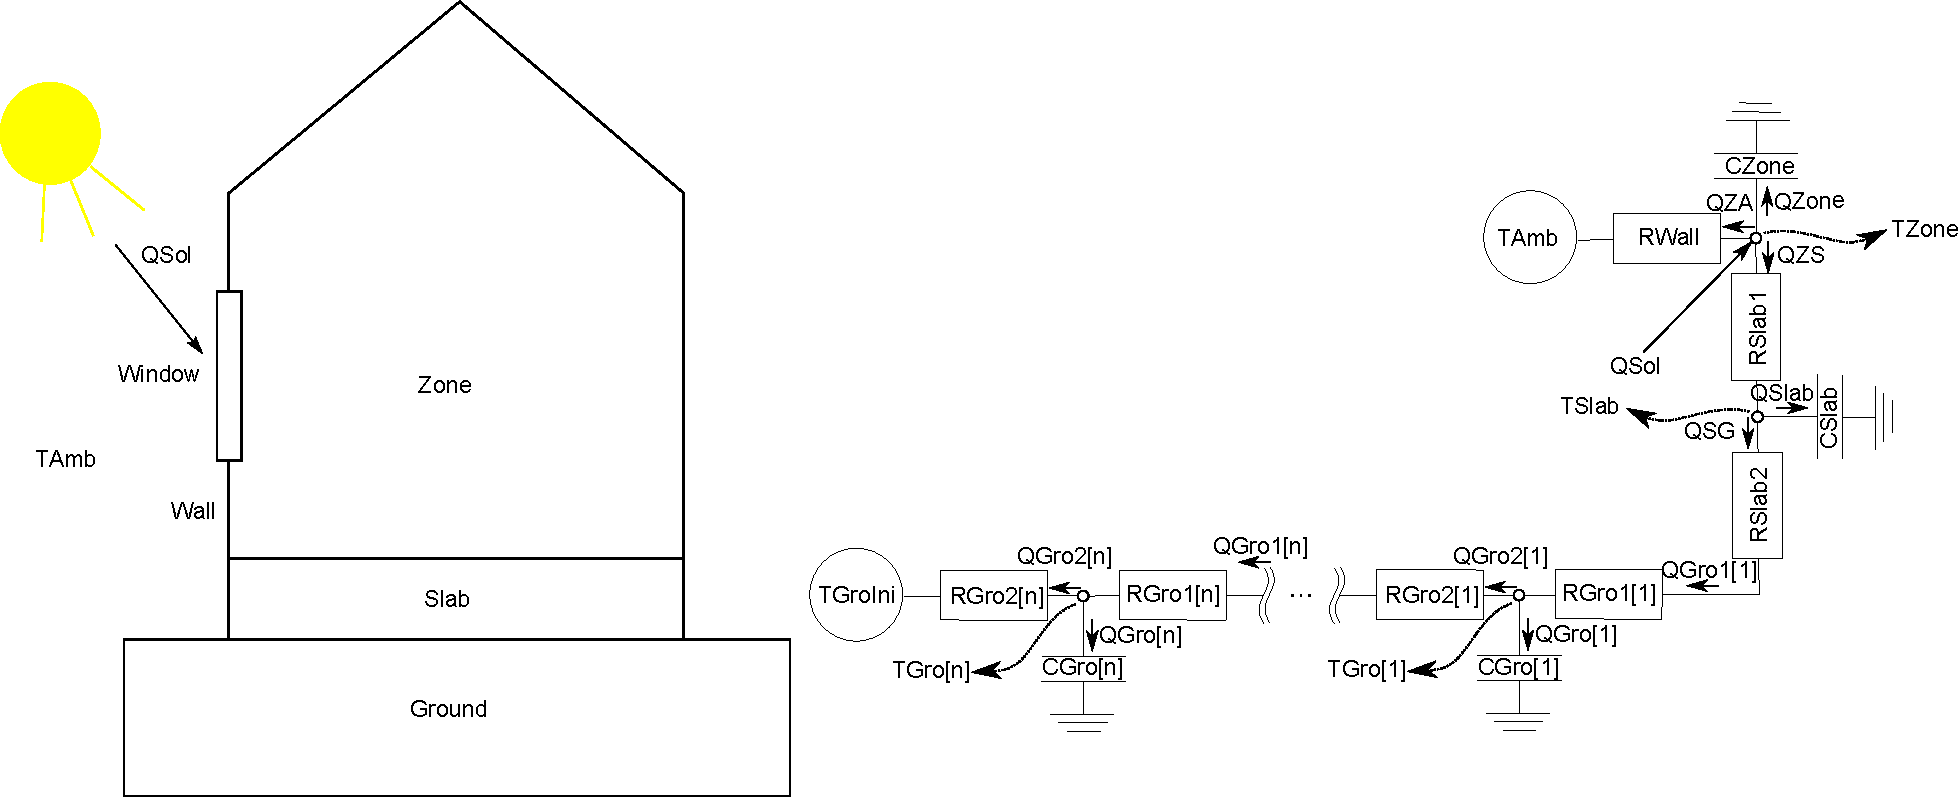
\includegraphics[width=1 \textwidth]{images/RCModelHouse.pdf}
	\caption{ Building model.}
	\label{fig:bui}
\end{figure}

\begin{table}[hbtp] 
\begin{tabular}{cccccc}
\hline 
  & RWall & RSlab1 & RSlab2 & RGro1[i] & RGro2[i] \\  
Thermal resistance $[K/W]$ & 0.00806 & 0.016 & 0.016 & 0.033 & 0.033 \\ 
\hline\hline 
  & CZone & CSlab & CGro[i] &   &   \\  
Thermal capacities $[J/K]$ & $2.4096 * 10^8$ & $3.36 * 10^8$ & $2.52*10^8$ &   &   \\ 
\hline\hline
  & TGroIni & TGro[i](start) & TSlab(start) & TZone(start)&  \\  
Temperature $[K]$ &  283.15 & 283.15 & 293.15 & 293.15 & \\ 
\hline 
\end{tabular} 
\caption{ Building parameters.}
\label{tab:par}
\end{table}

\textbf{Thermal resistance}: $T_1 - T_2 = \text{R} \ Q_{1 \rightarrow 2} $ with $R$ the thermal resistance between node 1 and 2 and $Q_{1\rightarrow 2}$ the heat flow, positive defined from 1 to 2.

\textbf{Thermal capacity}: $C \frac{\text{dT}}{dt} = Q$ with $C$ the thermal capacity and $Q$ the heat flow, positive defined flowing to the capacity.

\textbf{Conservation of energy (Kirchhoff)}: $ \sum Q_i = 0$ or the sum of the heat flows through one node is zero.

\subsection*{Questions}

\begin{enumerate}
\item Apply what you have learned during your reading by setting up a model for the building using the above mentioned equations. Approximate the ambient temperature by a sine using following code: $TAmb = 10*\cos(2*3.14*\text{time}*3*10^\wedge(-8)) + 276.15$ and the solar radiation by a trimmed cosine using: $QSol = \text{floor}(cos(2*\text{Modelica.Constants.pi}*\text{time} / 86400) + 1) * 5000 * cos(2*\text{Modelica.Constants.pi*time} / 86400)$. What is the zone temperature after a year under these conditions?
\item (OPTIONAL): Try to obtain the same results using the components of the Modelica library instead of writting the equations yourself. This library is automatically loaded in Dymola and can be found on the left-hand side of the dymola window. For thermal components, look in the Library at Modelica.Thermal.HeatTransfer.Components.   \linebreak[10]
\end{enumerate}

\begin{center}
 \textbf{Good luck!}
\end{center}

\end{document}
